% Sandia National Laboratories is a multimission laboratory managed and
% operated by National Technology & Engineering Solutions of Sandia, LLC, a
% wholly owned subsidiary of Honeywell International Inc., for the U.S.
% Department of Energy’s National Nuclear Security Administration under
% contract DE-NA0003525.

% Copyright 2002-2022 National Technology & Engineering Solutions of Sandia,
% LLC (NTESS).


\begin{Device}

\symbol
{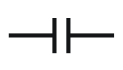
\includegraphics{capacitorSymbol}}

\device
\begin{alltt}
C<device name> <(+) node> <(-) node> [model name] [value]
+ [device parameters]
\end{alltt}

\model
\begin{alltt}
.MODEL <model name> C [model parameters]
.MODEL <model name> CAP [model parameters]
\end{alltt}

\examples
\begin{alltt}
CM12 2 4 5.288e-13
CLOAD 1 0 4.540pF IC=1.5V
CFEEDBACK 2 0 CMOD 1.0pF
CAGED 2 3 4.0uF D=0.0233 AGE=86200
CSOLDEP 3 0 C=\{ca*(c0+c1*tanh((V(3,0)-v0)/v1))\}
CSOLDEPQ 3 0 Q=\{ca*(c1*v1*ln(cosh((v(3,0)-v0)/v1))+c0*v(3,0))\}
\end{alltt}

\parameters
\begin{Parameters}
\param{device name}
The name of the device.

\param{\vbox{\hbox{(+) node\hfil}\hbox{(-) node}}}
Polarity definition for a positive voltage across the capacitor. The first
node is defined as positive. Therefore, the voltage across the component is
the first node voltage minus the second node voltage.

\param{model name}
If \texttt{model name} is omitted, then \texttt{value} is the capacitance in
farads.  If [model name] is given then the value is determined from the model
parameters; see the capacitor value formula below.

\param{value}
Positional specification of device parameter C (capacitance).  Alternately,
this can be specified as a parameter, \texttt{C=<value>}, or in the (optional)
model.

\param{device parameters}
Parameters listed in Table~\ref{C_1_Device_Instance_Params} may be provided as
space separated \texttt{<parameter>=<value>} specifications as needed.  Any number
of parameters may be specified.

\param{model parameters}
Parameters listed in Table~\ref{C_1_Device_Model_Params} may be provided as
space separated \texttt{<parameter>=<value>} specifications as needed.  Any number
of parameters may be specified.

\end{Parameters}

\comments
Positive current flows through the capacitor from
the \texttt{(+)} node to the \texttt{(-)} node.  In general, capacitors should
have a positive capacitance value (\texttt{<value>} property). In all cases,
the capacitance must not be zero.  

However, cases exist when a negative capacitance value may be used. This occurs
most often in filter designs that analyze an RLC circuit equivalent to a real
circuit. When transforming from the real to the RLC equivalent, the result may
contain a negative capacitance value.

In a transient run, negative capacitance values may cause the simulation to
fail due to instabilities they cause in the time integration
algorithms.

The power stored or released from the capacitor is calculated 
with $I \cdot \Delta V$ where the voltage drop is calculated as $(V_+ - V_-)$ 
and positive current flows from $V_+$ to $V_-$.

For compatibility with PSpice, either \texttt{C} or \texttt{CAP} can be used in a
\texttt{.MODEL} statement for a capacitor. 

The Multiplicity Factor (M) can be used to specify multiple, identical capacitors
in parallel. The effective capacitance becomes C*M. The M value need not be an
integer. It can be any positive real number. M can not be used as a model
parameter.

\end{Device}

\paragraph{Device Parameters}

% This table was generated by Xyce:
%   Xyce -doc C 1
%
\index{capacitor!device instance parameters}
\begin{DeviceParamTableGenerated}{Capacitor Device Instance Parameters}{C_1_Device_Instance_Params}
AGE & Age of capacitor & hour & 0 \\ \hline
C & Capacitance & F & 1e-06 \\ \hline
D & Age degradation coefficient & -- & 0.0233 \\ \hline
IC & Initial voltage drop across device & V & 0 \\ \hline
L & Semiconductor capacitor width & m & 1 \\ \hline
M & Multiplicity Factor & -- & 1 \\ \hline
Q & Charge & C & 0 \\ \hline
TC1 & Linear Temperature Coefficient & $^\circ$C$^{-1}$ & 0 \\ \hline
TC2 & Quadratic Temperature Coefficient & $^\circ$C$^{-2}$ & 0 \\ \hline
TEMP & Device temperature & $^\circ$C & Ambient Temperature \\ \hline
W & Semiconductor capacitor length & m & 1e-06 \\ \hline
\end{DeviceParamTableGenerated}


In addition to the parameters shown in the table, the capacitor supports a
vector parameter for the temperature correction coefficients.
\texttt{TC1=<linear coefficient>} and \texttt{TC2=<quadratic coefficient>} may
therefore be specified compactly as \texttt{TC=<linear coefficient>,<quadratic
coefficient>}.

\paragraph{Model Parameters}

% This table was generated by Xyce:
%   Xyce -doc C 1
%
\index{capacitor!device model parameters}
\begin{DeviceParamTableGenerated}{Capacitor Device Model Parameters}{C_1_Device_Model_Params}
C & Capacitance multiplier & -- & 1 \\ \hline
CJ & Junction bottom capacitance & F/m$^{2}$ & 0 \\ \hline
CJSW & Junction sidewall capacitance & F/m & 0 \\ \hline
DEFW & Default device width & m & 1e-06 \\ \hline
NARROW & Narrowing due to side etching & m & 0 \\ \hline
TC1 & Linear temperature coefficient & $^\circ$C$^{-1}$ & 0 \\ \hline
TC2 & Quadratic temperature coefficient & $^\circ$C$^{-2}$ & 0 \\ \hline
TNOM & Nominal device temperature & $^\circ$C & Ambient Temperature \\ \hline
\end{DeviceParamTableGenerated}


\paragraph{Capacitor Equations}

\subparagraph{Capacitance Value Formula}
If \texttt{[model name]} is specified, then the capacitance is given by:

\[
 \mathbf{C} \cdot (1 + \mathbf{TC1} \cdot (T - T_0) +
\mathbf{TC2} \cdot (T - T_0)^2)
\]
where \texttt{C} is the base capacitance specified on the device line
and is normally positive (though it can be negative, but not zero).
$T_0$ is the nominal temperature (set using \textrmb{TNOM} option).

\subparagraph{Age-aware Formula}
If \textrmb{AGE} is given, then the capacitance is:
\[\mathbf{C}[1 - \mathbf{D} \log(\mathbf{AGE})]\]

\subparagraph{Semiconductor Formula}
If \texttt{[model name]} and \textrmb{L} and \textrmb{W} are given, then the capacitance is:
\[
\mathbf{CJ}(\mathbf{L} - \mathbf{NARROW})(\mathbf{W} - \mathbf{NARROW}) + 2
\cdot \mathbf{CJSW}(\mathbf{L} - \mathbf{W} + 2 \cdot \mathbf{NARROW})
\]

\subparagraph{Solution-Dependent Capacitor}
If the capacitance (\texttt{C}) is set equal to an expression then a
``solution-dependent'' capacitor is used, where the capacitance is
a function of other simulation variables.  The formulas for
temperature-dependence and age-dependence, given above, then use that
calculated \texttt{C} value.

If the parameter \texttt{Q} is set equal to an expression {\em
  instead} of specifying a capacitance, this expression is used to
evaluate the charge on the capacitor instead of computing it from
capacitance.  Temperature and age dependence are not computed in this
case, as these effects are applied by modifying the capacitance.

Both solution-dependent charge and capacitance formulations are
implemented to assure charge conservation.  The capacitor:
\begin{alltt}
  c\_mcap 1 2 q=\{ca*(c1*v1*ln(cosh((v(1,2)-v0)/v1))+c0*v(1,2))\}
\end{alltt}
is exactly equivalent to the capacitor
\begin{alltt}
  c\_mcap 1 2 c=\{ca*(c0+c1*tanh((V(1,2)-v0)/v1))\}
\end{alltt}
because the capacitance is the derivative of the charge with respect
to the voltage drop across the capacitor.  Similarly, both are
equivalent to the behavioral source:
\begin{alltt}
  BC 1 2 I={ddt(V(1,2))*(ca*(c0+c1*tanh((V(1,2)-v0)/v1)))}
\end{alltt}
because $I=dQ/dt=dQ/dV*dV/dt=C*dV/dt$.

The restrictions for this formulation are:
\begin{XyceItemize}
  \item The expression used for \texttt{C} or \texttt{Q} must only use
    solution variables, which are node voltages and also branch
    currents for source devices.  It may not use device lead currents,
    which are post-processed quantities that are not solution variables.
  \item The expression must not use time derivatives.
  \item Capacitance (\texttt{C}) and Charge (\texttt{Q}) are the only
    instance or model parameters that are allowed to be
    solution-dependent.
\end{XyceItemize}

\paragraph{Other Restrictions and Caveats}
A netlist parsing error will occur if:
\begin{XyceItemize}
  \item Neither the \texttt{C}, \texttt{Q}, nor \texttt{L} instance
    parameters are specified.
  \item Both \texttt{C} and \texttt{Q} are specified as expressions.
    \item \texttt{Q} is specified in addition to an \texttt{IC=}.
  \item The \texttt{A} instance parameter is specified for a semiconductor 
      capacitor (which is specified via \texttt{L}, \texttt{W} and \texttt{CJSW}).
\end{XyceItemize}
If both the \texttt{C} and \texttt{L} instance parameters are specified then 
\texttt{C} will be used, rather than the semiconductor formulation. 

\paragraph{Special note on Initial Conditions:}

The IC parameter of the capacitor may be used to specify an initial
voltage drop on the capacitor.  Unlike SPICE3F5, this parameter is
never ignored (SPICE3F5 only respects it if UIC is used on a transient
line).  The initial condition is applied differently depending on the
analysis specified.

If one is doing a transient with DC operating point calculation or a
DC operating point analysis, the initial condition is applied by
inserting a voltage source across the capacitor to force the operating
point to find a solution with the capacitor charged to the specific
voltage.  The resulting operating point will be one that is consistent
with the capacitor having the given voltage in steady state.

If one specifies \texttt{UIC} or \texttt{NOOP} on the \texttt{.TRAN}
line, then \Xyce{} does not perform an operating point calculation,
but rather begins a transient simulation directly given an initial
state for the solution.  In this case, \texttt{IC} initial conditions
are applied only for the first iteration of the Newton solve of the
first time step --- the capacitor uses the initial condition to
compute its charge, and the nonlinear solver will therefore find a
solution to the circuit problem consistent with this charge, i.e., one
with the correct voltage drop across the capacitor.

The caveats of this section apply only to initial conditions specified
via \texttt{IC=} parameters on the capacitor, and do not affect how
initial conditions are applied when using \texttt{.IC} lines to
specify initial conditions on node values.

The three different ways of specifying initial conditions can lead to
different circuit behaviors.  Notably, when applying initial
conditions during a DC operating point with \texttt{IC=} on the
capacitor line, the resulting operating point will be a DC solution
with currents everywhere consistent with there being a constant charge
on the capacitor, whereas in general a transient run from an initial
condition {\em without\/} having performed an operating point
calculation will have a quiescent circuit at the first timestep.
